\documentclass{article}

\usepackage{geometry}
\usepackage{listings}
\geometry{a4paper, margin=1in}
\usepackage{amsmath}
\usepackage{graphicx	}
\usepackage[toc,page]{appendix}
\usepackage{caption}
\usepackage{subcaption}
\graphicspath{{./}}
\title{\textbf{Intro to Computer Vision \\Lab-7}\vfill{}}

\author{\textbf{Submitted By:}\\Saroj Kumar Dash}

\begin{document}
	\begin{titlepage}
		\maketitle
		\pagenumbering{gobble}
	\end{titlepage}
	
\newpage

\tableofcontents

\newpage	

\pagenumbering{arabic}
\textsl{•}\section{Introduction}
\paragraph{Camera Calibration}
Often in camera that captures the images has some distortion due to the lens and materials used in it. These distortions can be corrected using camera calibration in which we estimate the lens and camera distortions to correct the coordinates to obtain the image or the objects real world coordinates with respect to the camera. There are various methods to obtain this camera calibration parameters in this experiment we use the Tsai camera model and clibration technique to measure the parameters of the camera calibration to obtain the world coordinates of the objects in the experiment and then track them in our tracking area. For this we use two sofwtares deveoped by Dr. Hoover and his team. The two sofwtares that we used for this experiment is Calibration.exe and OccMap.exe, where Calibration.exe was used for calibration and OccMap.exe was used to check my caibration. The steps that I followed to calibrate and test is mentioned in the following section.

\section{Method and Results}
For this I used the camera network in the Riggs 13/15/17 lab. I followed the below steps to do the experiment to caibration of the camera.
\paragraph{Calibration steps:}
In the lab computer I used the Calibration.exe software to do this experiment. 
\begin{enumerate}
\item First I took 6 calibration targets and spread it on the floor to make a grid. I took a target with a cross made on it instead of a square to identify it as a marker for my chosen origin(0,0) in the world coordinates.I also decided my X-axis and Y-axis in the grid to map it in the calibration software. I took the small axis from my orgin as x-axis and the long axis as Y-axis. Below are my calibrate images that I took. The calbration.exe recognized my grid as a 4x6 matrix and then asked few questions to make sure of the coordinates that it recognized and also the direction of x-axis and y-axis.Below are the images and the coordinates that it recognised in my case.:
\begin{figure}[!htb]
    \centering
  		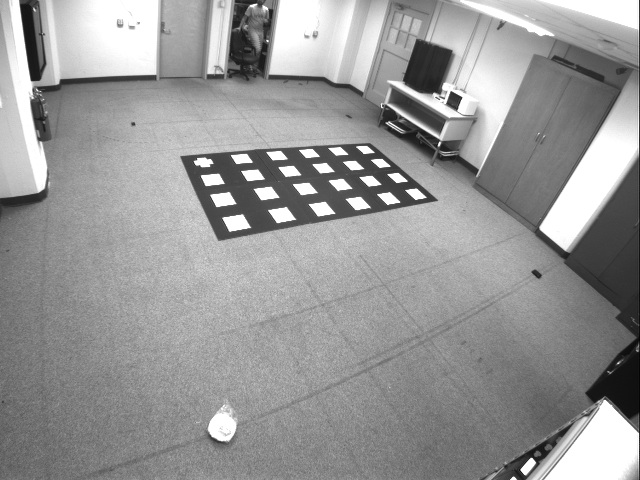
\includegraphics[scale=0.6]{CalImage_0.png}
  		\caption{Cam 0, the shorter side is X-Axis and the longer side is Y-axis}
  		\label{Fig1}
 \end{figure}

\newpage
\begin{figure}[!htb]
    \centering
  		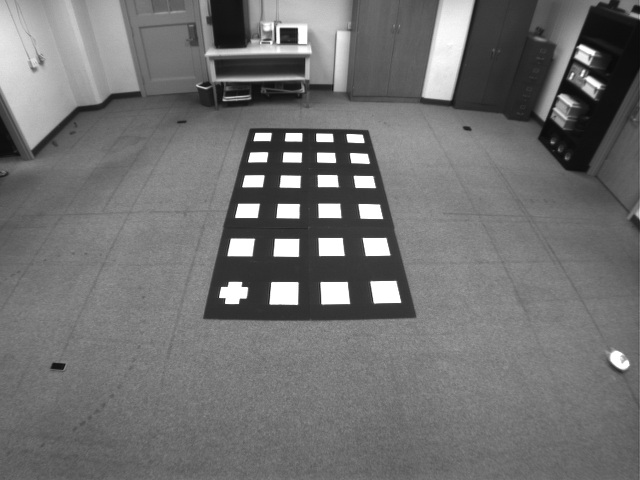
\includegraphics[scale=0.6]{CalImage_1.png}
  		\caption{Cam 1}
  		\label{Fig2}
 \end{figure}

\begin{figure}[!htb]
    \centering
  		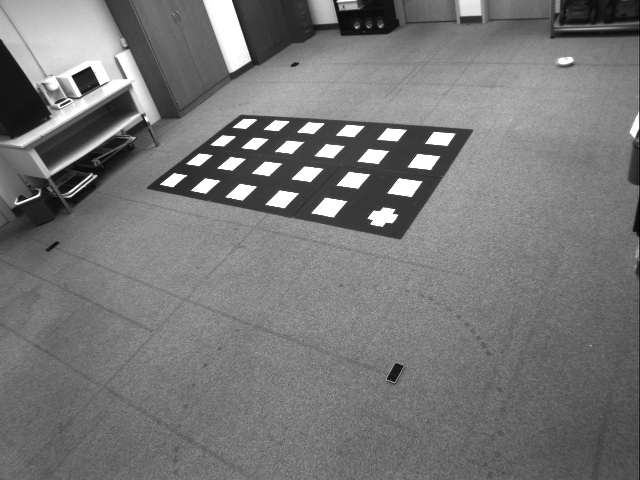
\includegraphics[scale=0.6]{CalImage_2.png}
  		\caption{Cam 2}
  		\label{Fig3}
 \end{figure}

\begin{figure}[!htb]
    \centering
  		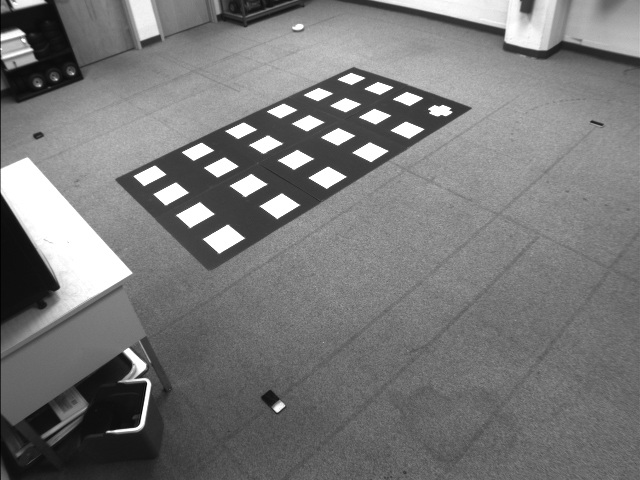
\includegraphics[scale=0.6]{CalImage_3.png}
  		\caption{Cam 3}
  		\label{Fig4}
 \end{figure}

\newpage
\begin{figure}[!htb]
    \centering
  		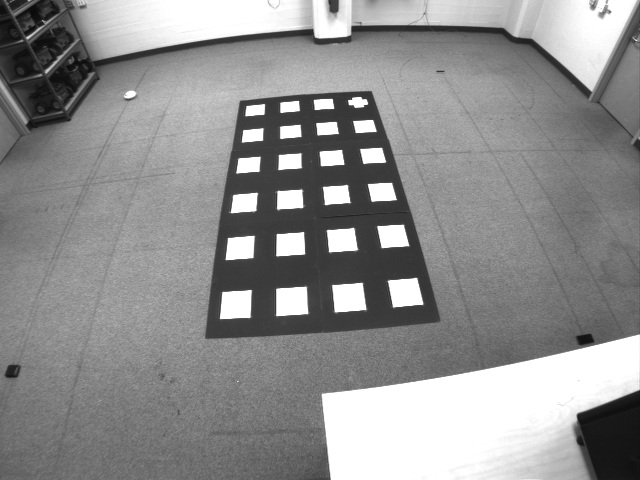
\includegraphics[scale=0.6]{CalImage_4.png}
  		\caption{Cam 4}
  		\label{Fig5}
 \end{figure}
\newpage
 \begin{figure}[!htb]
    \centering
  		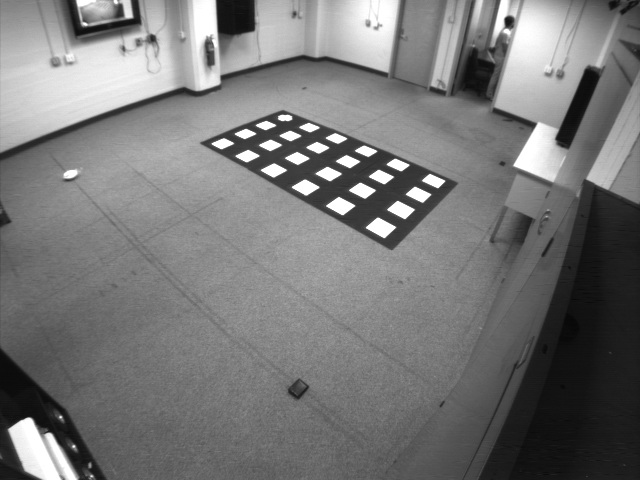
\includegraphics[scale=0.6]{CalImage_5.png}
  		\caption{Cam 5}
  		\label{Fig6}
 \end{figure}

Using the above images I got the coordinates which are shown in the table mentioned below. The screenshot for the cam 0 is displayed below. 
\begin{center}
 \begin{tabular}{||c c c c||} 
 \hline
 Cam & X & Y & Z \\ [0.5ex] 
 \hline\hline
 0 & 3889 & -1197 & 2333 \\ 
 \hline
 1 & 593 & -1736 & 2270 \\
 \hline
 2 & -2181 & -1484 & 2022 \\
 \hline
 3 & -2553 & 3721 & 2316 \\
 \hline
 4 & 586 & 3784 & 2282 \\  
 \hline
 5 & 3753 & 3712 & 2280 \\ [1ex] 
 \hline
\end{tabular}
\end{center}

\newpage
Image or screenshot of the coordinates that I got from cam-0.
\begin{figure}[!htb]
    \centering
  		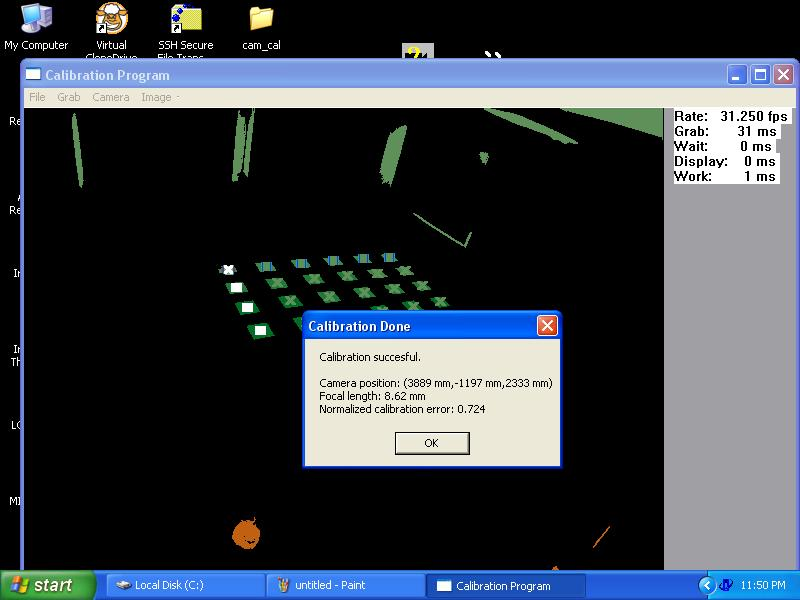
\includegraphics[scale=0.6]{cam0.JPG}
  		\caption{screenshot of the coordinates that I obtain. This is only for the cam0. I got similar screenshots for all the rest of the 5 cameras.}
  		\label{Fig7}
 \end{figure}

\item After calibration of the coordinates, I removed the grids spread on the floor to capture the background image which will be used for the tracking of our object in the rectangular area. As shown in the image following we placed four objects at the corners of our imaginary boundary of the tracking area to keep track of the area which should be calibrated for the tracking area. In the process we took a snapshot from the camera and draw my cotours around the imaginary backgrund area of tracking, below are the 6 background images that we captured and also the corresponding floor.txt files which shows our points to snap the background image of the floor.
\newpage
\begin{figure}[!htb]
    \centering
  		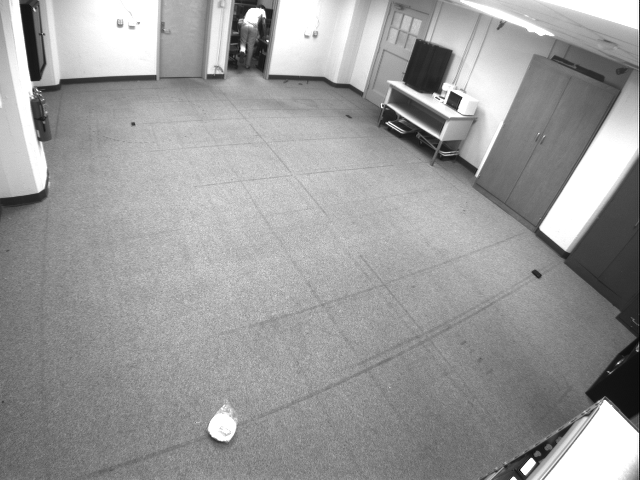
\includegraphics[scale=0.6]{Background0.png}
  		\caption{screenshot of the coordinates that I obtain. This is only for the cam0. I got similar screenshots for all the rest of the 5 cameras.}
  		\label{Fig8} 
 \end{figure} 
Contents from  the file $Floor_0.txt$ which represents the points that I captured for drawing the contours.
\lstinputlisting{Floor_0.txt}

\begin{figure}[!htb]
    \centering
  		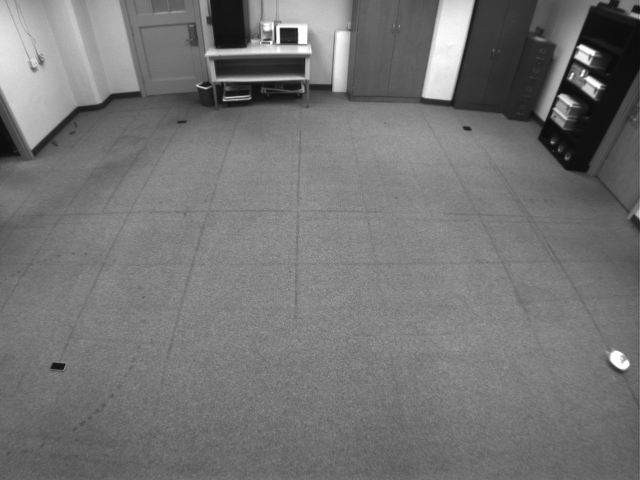
\includegraphics[scale=0.5]{Background1.png}
  		\caption{ Cam 1\\}
  		\label{Fig9}
 \end{figure}
Contents from  the file $Floor_1.txt$ which represents the points that I captured for drawing the contours.
\lstinputlisting{Floor_1.txt}

\newpage
\begin{figure}[!htb]
    \centering
  		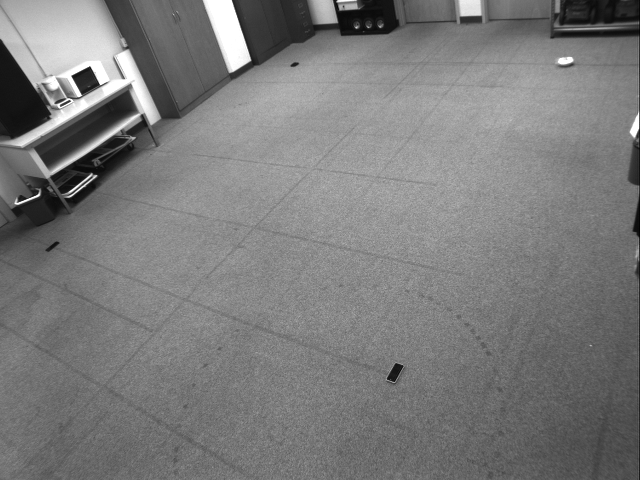
\includegraphics[scale=0.5]{Background2.png}
  		\caption{ Cam 2\\}
  \end{figure}
Contents from  the file $Floor_2.txt$ which represents the points that I captured for drawing the contours.
\lstinputlisting{Floor_2.txt}

\begin{figure}[!htb]
    \centering
  		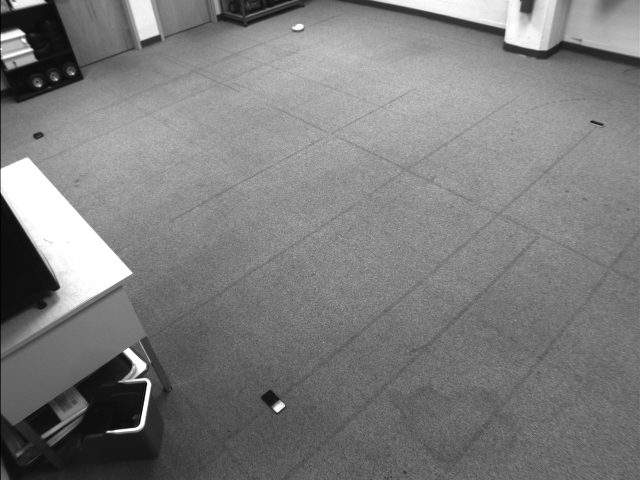
\includegraphics[scale=0.5]{Background3.png}
  		\caption{ Cam 3\\}
  \end{figure}
Contents from  the file $Floor_3.txt$ which represents the points that I captured for drawing the contours.
\lstinputlisting{Floor_3.txt}

\newpage
\begin{figure}[!htb]
    \centering
  		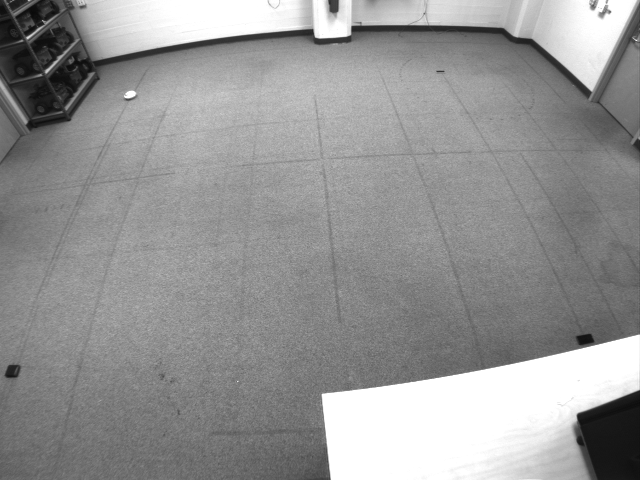
\includegraphics[scale=0.5]{Background4.png}
  		\caption{ Cam 4}
 \end{figure}
Contents from  the file $Floor_4.txt$ which represents the points that I captured for drawing the contours.
\lstinputlisting{Floor_4.txt}

\begin{figure}[!htb]
    \centering
  		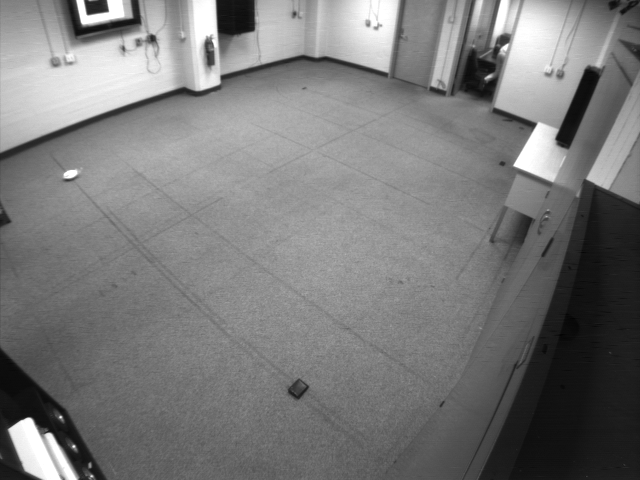
\includegraphics[scale=0.5]{Background5.png}
  		\caption{ Cam 5}
 \end{figure}
Contents from  the file $Floor_5.txt$ which represents the points that I captured for drawing the contours.
\lstinputlisting{Floor_5.txt}

\item After the calibration and background images were recognized. All the data was used to test my tracking. I opened the OccMap.exe application and I found a rectangular area for tracking and then used a chair in the lab to push into the tracking area and I successfully found it with no shadows in it proving that the images or camera feed all the cameras are considered and is displayed.
\begin{figure}[!htb]
    \centering
  		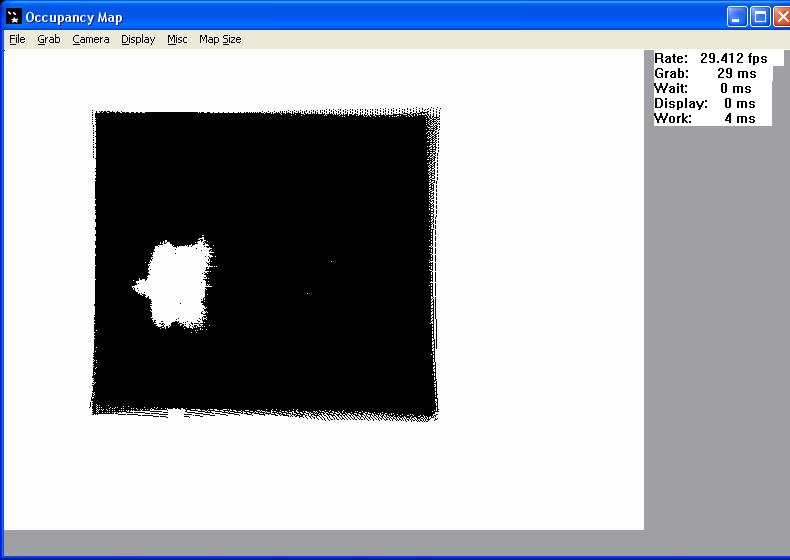
\includegraphics[scale=0.5]{ocm.JPG}
  		\caption{ Final Result. Chair blob is obtained in my tracking area.}
 \end{figure}

\end{enumerate}

\newpage
\section{Conclusion}
In the Lab I learnt the techniques on how to use a check grid system to do the camera calibration.I also learnt how to check if my camera calibration is showing correct result or not.
\newpage
\section{Appendix}
\lstinputlisting[caption=$Calib_0.txt$]{Calib_0.txt}
\lstinputlisting[caption=$Calib_1.txt$]{Calib_1.txt}
\lstinputlisting[caption=$Calib_2.txt$]{Calib_2.txt}
\lstinputlisting[caption=$Calib_3.txt$]{Calib_3.txt}
\lstinputlisting[caption=$Calib_4.txt$]{Calib_4.txt}
\newpage
\lstinputlisting[caption=$Calib_5.txt$]{Calib_5.txt}
\lstinputlisting[caption=$CalPoints_0.txt$]{CalPoints_0.txt}
\lstinputlisting[caption=$CalPoints_1.txt$]{CalPoints_1.txt}
\lstinputlisting[caption=$CalPoints_2.txt$]{CalPoints_2.txt}
\lstinputlisting[caption=$CalPoints_3.txt$]{CalPoints_3.txt}
\lstinputlisting[caption=$CalPoints_4.txt$]{CalPoints_4.txt}
\lstinputlisting[caption=$CalPoints_5.txt$]{CalPoints_5.txt}
\label{appendix: Appendix A}
\end{document}